\documentclass[tikz]{standalone}
\usetikzlibrary{math,shapes.geometric,calc,positioning}

\begin{document}
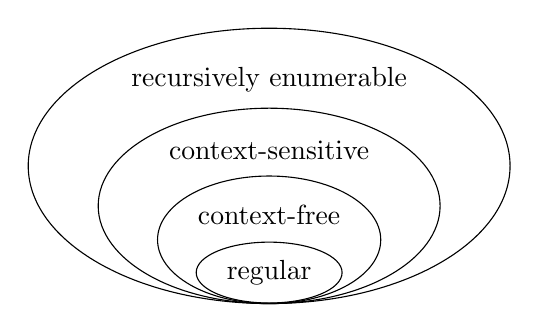
\begin{tikzpicture}[xscale=3.5,yscale=2]
	
	\coordinate (zero) at (0,0);
	
	\node [ellipse,above=0pt of zero,draw] (regular) {regular};
		\coordinate (regular-top) at ($(regular.north)$);
	
	%%%%%%%%%%%%%%%%%%%%%%%%%%%%%%%%%%%%%%%%%%%%%%%%%%%%%%
	
	\node [above=0.25em of regular-top] (context-free-text) {context-free};
	
	\draw [inner sep=0pt,outer sep=0pt,draw] let
	\p1=($(context-free-text.north)$),
	\p2=($(context-free-text.east)$),
	\n1={\x2/sin(180 - 2*atan2(\y1,\x2))}
	in
	(0,\n1) circle (\n1);
	%
	\path let
	\p1=($(context-free-text.north)$),
	\p2=($(context-free-text.east)$),
	\n1={\x2/sin(180 - 2*atan2(\y1,\x2))}
	in coordinate
	(context-free-top) at (0,2*\n1);
	
	%%%%%%%%%%%%%%%%%%%%%%%%%%%%%%%%%%%%%%%%%%%%%%%%%%%%%%
	
	
	\node [above=0.25em of context-free-top] (context-sensitive-text) {context-sensitive};
	
	\draw [inner sep=0pt,outer sep=0pt,draw] let
	\p1=($(context-sensitive-text.north)$),
	\p2=($(context-sensitive-text.east)$),
	\n1={\x2/sin(180-2*atan2(\x2,\y1))}
	in
	(0,\n1) circle (\n1);
	%
	\path let
	\p1=($(context-sensitive-text.north)$),
	\p2=($(context-sensitive-text.east)$),
	\n1={\x2/sin(180-2*atan2(\x2,\y1))}
	in coordinate
	(context-sensitive-top) at (0,2*\n1);
		
	%%%%%%%%%%%%%%%%%%%%%%%%%%%%%%%%%%%%%%%%%%%%%%%%%%%%%%
	
	\node [above=0.25em of context-sensitive-top] (re-text) {recursively enumerable};
	
	\draw [inner sep=0pt,outer sep=0pt,draw] let
	\p1=($(re-text.north)$),
	\p2=($(re-text.east)$),
	\n1={\x2/sin(180 - 2*atan2(\y1,\x2))}
	in
	(0,\n1) circle (\n1);
	%
	\path let
	\p1=($(re-text.north)$),
	\p2=($(re-text.east)$),
	\n1={\x2/sin(180 - 2*atan2(\y1,\x2))}
	in coordinate
	(re-top) at (0,2*\n1);
	
\end{tikzpicture}
\end{document}
